\chapter{FPGA Implementation}\label{chap:FPGA_Implementation}

\section{About}\label{sec:About}
The Chipyard Framework contains initial support for \gls{fpga} development and simulation of \gls{soc} designs.
At the moment this support is very limited, and is in active development.
As of \today, the best support for FPGA Development for the Arty 35T FPGA comes from a branch of Chipyard called \href{https://github.com/ucb-bar/chipyard/tree/arty-spi-flash}{arty-spi-flash}.
This branch fixes the \gls{uart} implementation, and enables the \gls{spi} flash storage on the Arty FPGA to allow users to store programs on the FPGA.

\section{Prerequisites}\label{sec:Prerequisites}
To assist with the proper setup, we approached the FPGA implementation of an SoC by following the ``SiFive Freedom E310 Arty FPGA Dev Kit Getting Started Guide''~\cite{FreedomDevGuide}.
This outlined many of the steps we would eventually need to take, starting with purchasing an \href{https://www.digikey.com/en/products/detail/olimex-ltd/ARM-USB-TINY-H/3471388}{Olimex JTAG Debugger}~\cite{OlimexJTAG}.
Once the final image is flashed to the FPGA, the debugger will allow the user to upload C programs and execute them on the RISC-V processor.

\begin{figure}[h!tbp]
  \centering
  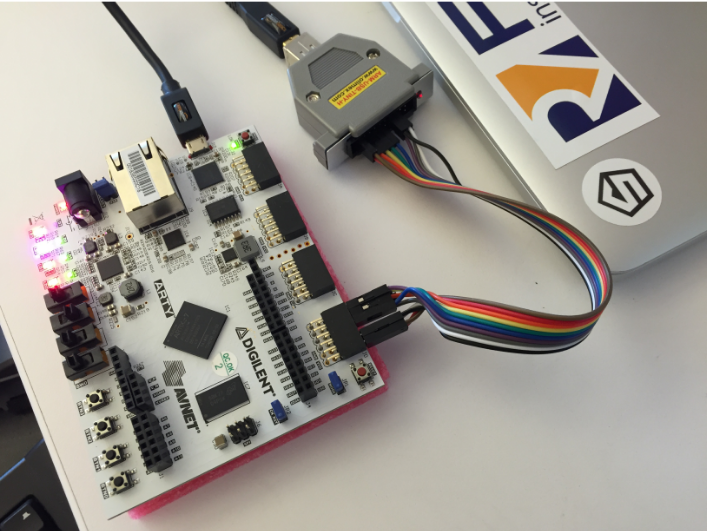
\includegraphics[width=0.7\linewidth]{./OlimexSetup.png}
  \caption{Olimex Debugger Setup~\cite[p.~5]{FreedomDevGuide}}
  \label{fig:olimexsetup}
\end{figure}

%%% Local Variables:
%%% mode: latex
%%% TeX-master: "../doc"
%%% End:
